\item A un disco de masa $M$ y radio $R$ se le saca un trozo concéntrico de radio $r$. Este disco está unido a dos resortes de constante elástica $k$ y gira respecto al eje que se indica en la siguiente figura de la izquierda, la figura de la derecha corresponde a otra vista del disco.

\begin{center}
	<div style='border:1px solid black;'>
		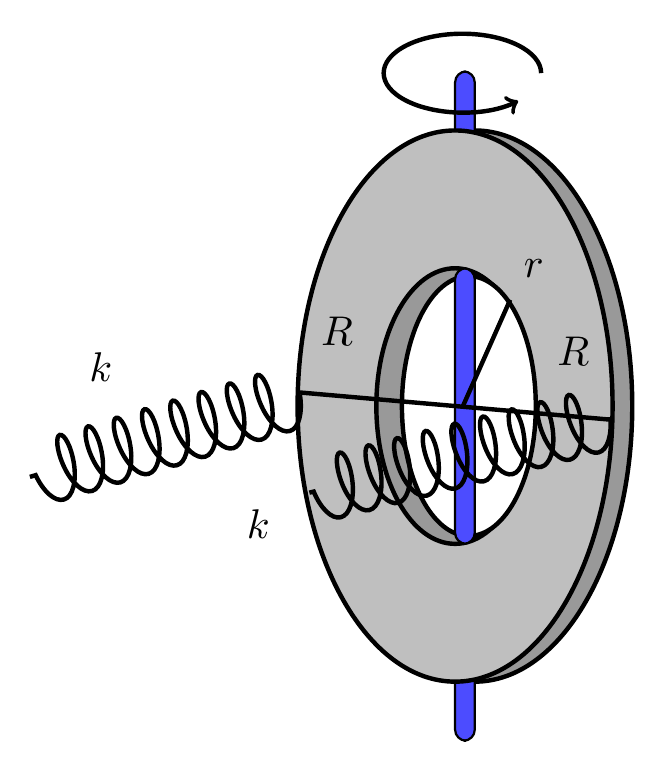
\begin{tikzpicture}[scale=1]
		%Disco 1%
		\filldraw [fill=white!20!gray, ultra thick] (.25,0) circle [x radius=2 ,y radius=3.5];
		\filldraw [thick, fill=white!30!blue,rounded corners] (-0,4.25)rectangle(.25,-4.25);
		\filldraw [fill=white!50!gray, ultra thick] (0,0) circle [x radius=2 ,y radius=3.5];
		\filldraw [fill=white!20!gray, ultra thick] (0,0) circle [x radius=1 ,y radius=1.75];
		\filldraw [fill=white, ultra thick] (.175,0) circle [x radius=.85 ,y radius=1.65];
		\filldraw [thick, fill=white!30!blue,rounded corners] (-0,1.75)rectangle(.25,-1.75);
		\draw [ultra thick,rotate=-5] (2,0)--(-2,0);
		\draw [ultra thick](.1,0)--(.7,1.35);
		\draw [ultra thick, decoration={aspect=0.4, segment length=3.75mm, amplitude=4mm, coil}, decorate] (-1.97,.14)--(-5.4,-.9);
		\draw [ultra thick, decoration={aspect=0.4, segment length=3.75mm, amplitude=4mm, coil}, decorate] (1.97,-.14)--(-1.85,-1.1);
		\draw[<-,ultra thick] (.8,3.875)  arc[x radius = 1, y radius = .5, start angle= 315, end angle= 0];
		\draw [dotted]
		(-1.5,.95) node[scale=1.5] {\(R\)}
		(1.5,.7) node[scale=1.5] {\(R\)}
		(1,1.75) node[scale=1.5] {\(r\)}
		(-4.5,.5) node[scale=1.5] {\(k\)}
		(-2.5,-1.5) node[scale=1.5] {\(k\)}
		;
		\end{tikzpicture}
		
		\hspace{20mm}
		
		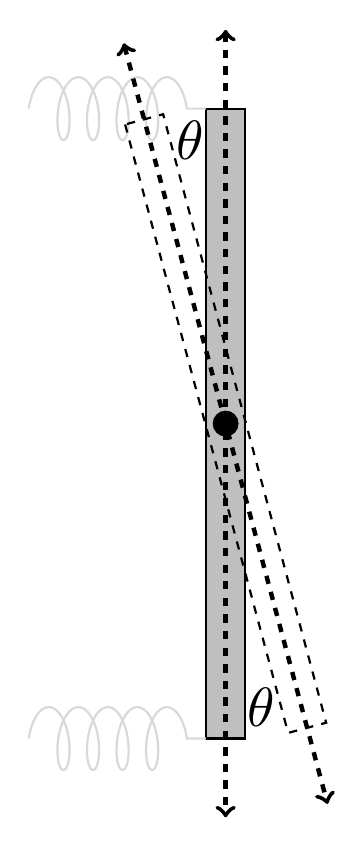
\begin{tikzpicture}[scale=1]
		%Disco2%
		\filldraw [thick, fill=white!50!gray] (-.25,4)rectangle(.25,-4);
		\filldraw [thick, fill=black] (0,0)circle(.15);
		\draw [dashed, <->,ultra thick] (0,5)--(0,-5);
		\draw [gray!30!white,thick, decoration={aspect=0.4, segment length=3.75mm, amplitude=4mm, coil}, decorate] (-2.5,4)--(-.25,4);
		\draw [gray!30!white,thick, decoration={aspect=0.4, segment length=3.75mm, amplitude=4mm, coil}, decorate] (-2.5,-4)--(-.25,-4);
		\draw [dashed,thick, rotate=15] (-.25,4)rectangle(.25,-4);
		\draw [dashed, <->,ultra thick,rotate=15] (0,5)--(0,-5);
		\draw [dotted] 
		(-.45,3.6) node[scale=2] {\(\theta\)}
		(.45,-3.6) node[scale=2] {\(\theta\)}
		;
		
		\end{tikzpicture}
		
	</div>
\end{center}

\begin{enumerate}[a)]
	\item Determine el momento de inercia $I$ del disco respecto al eje de giro del disco en función de las variables indicadas en el problema. El momento de inercia para un disco de radio $R$ y masa $M$ está dado por:
	
	\begin{center}
		<div style='border:1px solid black;'>
			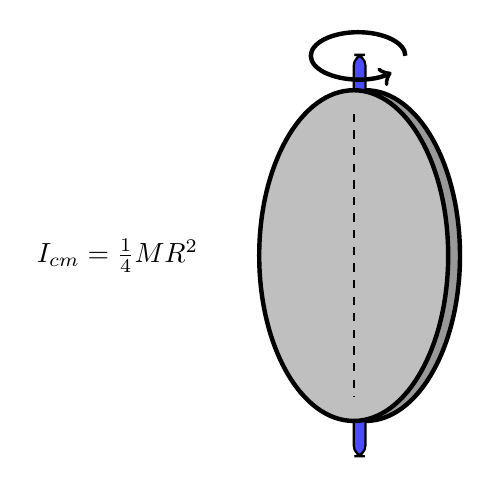
\begin{tikzpicture}[scale=.6]
			%DiscoAyuda%
			\filldraw [fill=white!20!gray, ultra thick] (.25,0) circle [x radius=2 ,y radius=3.5];
			\filldraw [thick, fill=white!30!blue,rounded corners] (-0,4.25)rectangle(.25,-4.25);
			\filldraw [fill=white!50!gray, ultra thick] (0,0) circle [x radius=2 ,y radius=3.5];
			\draw[<-,ultra thick] (.8,3.875)  arc[x radius = 1, y radius = .5, start angle= 315, end angle= 0];
			\draw [dashed, thick] (0,3)--(0,-3);
			\draw [dotted]
			(-5,0) node[scale=1] {\(I_{cm}=\frac{1}{4}MR^2\)}
			;
			\end{tikzpicture}
		</div>
	\end{center}
	
	El momento de inercia del sistema, respecto al eje de giro mostrado en la figura, está dado por la diferencia entre el momento de inercia del disco completo de masa $M$, menos el momento de inercia del disco concéntrico que es retirado, $$I=I_\text{CM}=\dfrac{1}{4}MR^2-\dfrac{1}{4}mr^2,$$
	donde $m$ corresponde a la masa de la sección retirada y se puede calcular, asumiendo la densidad superficial de masa del disco $\sigma$ constante, de la siguiente manera,$$\sigma=\frac{M}{\pi R^2}=\frac{m}{\pi r^2}\qquad\Rightarrow\qquad m=M \dfrac{r^2}{R^2}.$$ Luego, $$I=\frac{1}{4}M\left(R^2-\frac{r^4}{R^2}\right)\qquad\Rightarrow\qquad I=\frac{1}{4}M \left(\frac{R^4-r^4}{R^2}\right).$$
	
	\item Determine la ecuación de movimiento del disco en función de la variable $\theta$ que se indica en la figura para pequeñas oscilaciones.
	
	Usamos la segunda ley de Newton en su forma rotacional $\sum\vec\tau=I\vec\alpha$. Calculamos respecto al eje de giro mostrado en la figura para oscilaciones pequeñas, $$-k(R\theta)R-k(R\theta)R=I\ddot\theta.$$ Luego, $$\ddot\theta+\frac{2kR^2}{I}\theta=0\qquad\Rightarrow \qquad\ddot\theta+\frac{8k}{M}\left(\frac{R^4}{R^4-r^4}\right)\theta=0.$$
	
	\item Determine la frecuencia natural de oscilación $\omega_0$. del disco en función de las variables del problema.
	
	De la ecuación de movimiento, $$\omega_0=\sqrt{\frac{8k}{M}\left(\frac{R^4}{R^4-r^4}\right)}.$$
	
	Se ubica un amortiguador a una distancia $x$ desde el centro de giro como se muestra en la siguiente figura.
	
	\begin{center}
		<div style='border:1px solid black;'>
			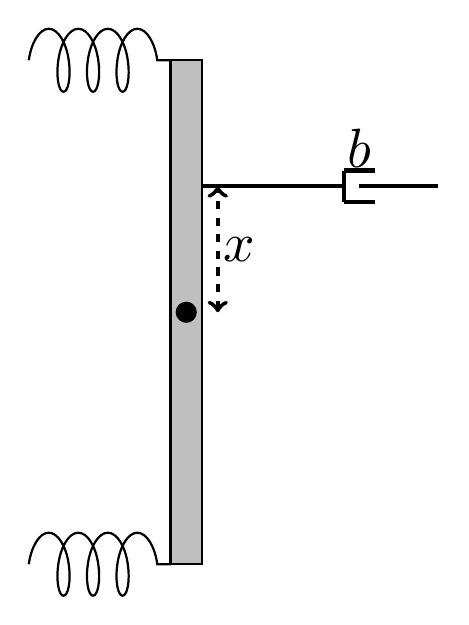
\begin{tikzpicture}[scale=.8]
			%Disco3%
			\filldraw [thick, fill=white!50!gray] (-.25,4)rectangle(.25,-4);
			\filldraw [thick, fill=black] (0,0)circle(.15);
			\draw [ultra thick] (.25,2)--(2.5,2) (2.5,2.25)--(2.5,1.75) (2.5,2.25)--(3,2.25) (2.5,1.75)--(3,1.75) (2.75,2)--(4,2);
			\draw [dashed, <->,ultra thick] (.5,0)--(.5,2);
			\draw [thick, decoration={aspect=0.4, segment length=3.75mm, amplitude=4mm, coil}, decorate] (-2.5,4)--(-.25,4);
			\draw [thick, decoration={aspect=0.4, segment length=3.75mm, amplitude=4mm, coil}, decorate] (-2.5,-4)--(-.25,-4);
			\draw [dotted] 
			(.85,1) node[scale=2] {\(x\)}
			(2.75,2.6) node[scale=2] {\(b\)}
			;
			\end{tikzpicture}
		</div>
	\end{center}
	
	\item ¿Qué valor debe tener $x$ para que sea un oscilador amortiguado crítico?
	
	El amortiguador ejerce una fuerza de amortiguamiento del tipo $bv$, donde $v=x\dot\theta$. Aplicamos nuevamente la segunda ley de Newton, $$-k(R\theta)R-k(R\theta)R-b(x\dot\theta)x=I\ddot\theta.$$ Luego,
	$$\ddot\theta+\frac{bx^2}{I}\dot\theta+\frac{2kR^2}{I}\theta=0.$$ Podemos asociar la constante de amortiguamiento a $$2\gamma=\frac{bx^2}{I},\qquad\text{as\'i}\qquad\gamma(x)=\frac{bx^2}{2I}.$$ La condición para que el movimiento sea críticamente amortiguado está dado por $\sqrt{\omega_0^2-\gamma^2}=0$, entonces, $\gamma(x)=\omega_0$. Despejando $x$ tenemos,
	$$x=\sqrt{\frac{2I\omega_0}{b}}\qquad\Rightarrow\qquad x=\sqrt{\frac{1}{b}} \ \sqrt[4]{2kM(R^4-r^4)}.$$
	
	\item Indique si puede ser $x<r$, justifique su respuesta.
	
	La única condición que debe satisfacer $x$ es que debe ser menor a $R$. Por otro lado, podemos colocar el amortiguador tal que $x<r$, siempre que esté conectado a una altura por encima, o por debajo, donde exista disco.
	
\end{enumerate}
